\documentclass[tikz,border=8pt]{standalone}
\usepackage{amsmath,amssymb}
\usetikzlibrary{arrows.meta,automata,positioning,quotes}
\begin{document}
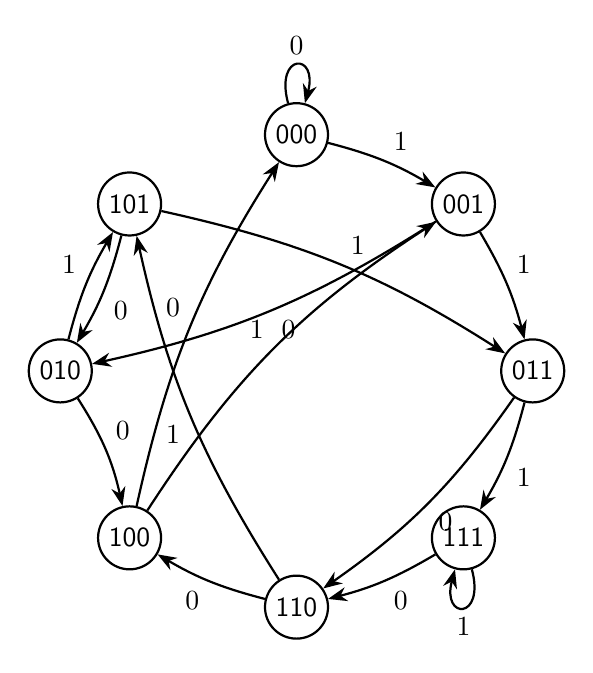
\begin{tikzpicture}[x=1cm,y=1cm]
\tikzset{
  graphnode/.style={circle,draw,thick,minimum size=8mm,inner sep=1pt,font=\sffamily},
  directed/.style={-{Stealth[length=2.4mm]},thick},
  undirected/.style={thick}
}
\node[graphnode] (n_v_000) at (0.00,3.00) {000};
\node[graphnode] (n_v_001) at (2.12,2.12) {001};
\node[graphnode] (n_v_010) at (-3.00,0.00) {010};
\node[graphnode] (n_v_011) at (3.00,0.00) {011};
\node[graphnode] (n_v_100) at (-2.12,-2.12) {100};
\node[graphnode] (n_v_101) at (-2.12,2.12) {101};
\node[graphnode] (n_v_110) at (0.00,-3.00) {110};
\node[graphnode] (n_v_111) at (2.12,-2.12) {111};
\draw[directed] (n_v_000) to[loop above, "0"] (n_v_000);
\draw[directed] (n_v_000) to[bend left=8, "1"] (n_v_001);
\draw[directed] (n_v_001) to[bend left=10, "0"] (n_v_010);
\draw[directed] (n_v_001) to[bend left=8, "1"] (n_v_011);
\draw[directed] (n_v_010) to[bend left=10, "0"] (n_v_100);
\draw[directed] (n_v_010) to[bend left=8, "1"] (n_v_101);
\draw[directed] (n_v_011) to[bend left=10, "0"] (n_v_110);
\draw[directed] (n_v_011) to[bend left=8, "1"] (n_v_111);
\draw[directed] (n_v_100) to[bend left=10, "0"] (n_v_000);
\draw[directed] (n_v_100) to[bend left=12, "1"] (n_v_001);
\draw[directed] (n_v_101) to[bend left=8, "0"] (n_v_010);
\draw[directed] (n_v_101) to[bend left=10, "1"] (n_v_011);
\draw[directed] (n_v_110) to[bend left=8, "0"] (n_v_100);
\draw[directed] (n_v_110) to[bend left=10, "1"] (n_v_101);
\draw[directed] (n_v_111) to[bend left=8, "0"] (n_v_110);
\draw[directed] (n_v_111) to[loop below, "1"] (n_v_111);
\end{tikzpicture}
\end{document}
